%
% 4-prinzipal.tex
%
% (c) 2024 Prof Dr Andreas Müller
%

%
% Prinzipalbündel
%
\section{Zusammenhang und Prinzipalbündel
\label{buch:fallstudie:prinzipalbuendel}}
\kopfrechts{Zusammenhang und Prinzipalbündel}%
Es gibt Vektorfelder, die nichts mit den Verschiebungsvektoren im
Definitionsbereich zu tun haben.
Ein Farbbild ordnet jedem Punkt der Bildebene einen dreidimensionalen
Vektor zu, der die Farbkomponenten $R$, $G$ und $B$ enthält.
In diesem Fall ist klar, dass die Verschiebung oder Drehung in der
Bildebene sich nicht auf die Farben auswirkt.

Auch die elektrischen und magnetischen Feldvektoren werden zwar
\index{elektrisches Feld}%
\index{magnetisches Feld}%
oft im gleichen Raum dargestellt, haben aber eigentlich nur indirekt
etwas mit den Raumdimensionen zu tun.
Aus dem elektrischen Feldvektor lässt sich durch Multiplikation die
Kraft berechnen, die das elektrische Feld auf eine Testladung ausübt,
die sich in Form der Beschleunigung der Ladung und der Krümmung der
Bahnkurve bemerkbar macht.
Es stellt sich aber spätestens in der speziellen Relativitätstheorie
heraus, dass das elektrische Potential $\varphi$ und das Vektorpotential
$\vec{A}$ die geeigneteren Grössen zur Beschreibung des elektromagnetischen
Feldes sind.
Die sogenannten Eichtransformationen sind zusätzliche Symmetrien, denen
\index{Eichtransformation}%
das aus $\varphi$ und $\vec{A}$ kombinierte Feld genügt.
Sie können interpretiert werden als eine Modifikation der
Ableitungsoperatoren, die ihrerseits mit den Verschiebungsvektoren
verbunden sind.

Auf gekrümmten Flächen ist es nicht selbstverständlich, einen
Tangentialvektor in einem Punkt mit einem Tangentialvektor in einem
Nachbarpunkt zu vergleichen.
Der Transport entlang einer Kurve in einer gekrümmten Fläche wirkt
sich daher auch auf den Transport von Tangentialvektoren aus.
Dies wirkt sich auf den Begriff der Ableitung aus.
Für den Vergleich ist ein sogenannter {\em Zusammenhang} notwendig, mit
dem sich die {\em kovariante Ableitung} konstruieren lässt.
\index{kovariante Ableitung}%
\index{Ableitung, kovariant}%
Ein ähnliches Phänomen tritt bei der Beschreibung von Strömungen
auf, wo Vektoren von der Strömung transportiert werden und dabei
verändert werden können.

%
% spin12.tex
%
% (c) 2024 Prof Dr Andreas Müller
%
\begin{figure}
\centering
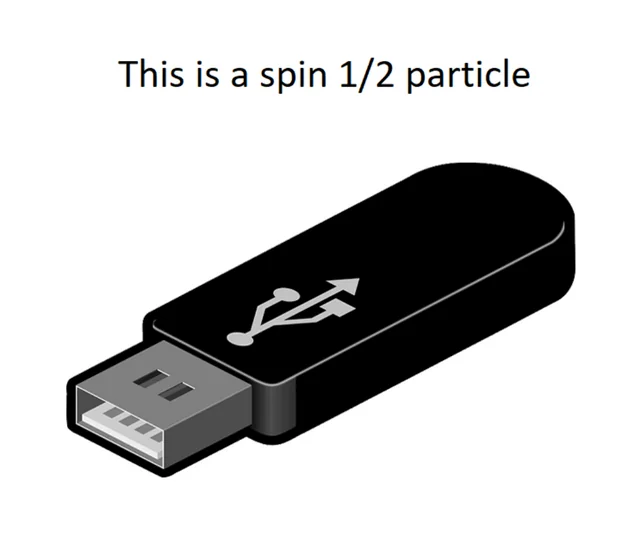
\includegraphics[width=8cm]{chapters/010-fallstudie/images/spin12.png}
\caption{Internet Meme, welches die frustrierende Erfahrung, dass sich
ein USB-Stick oft erst beim dritten oder vierten Versuch einstecken
lässt, scherzhaft als Spin-$\frac12$-Phänomen interpretiert.
\label{buch:fallstudie:fig:spin12}}
\end{figure}
%

Der Spin eines Elektrons ist eine Quanteneigenschaft, die mit der
\index{Elektron}%
\index{Spin}%
Drehung des Raums gekoppelt ist.
Da ein Elektron zwei mögliche Spin-Orientierungen haben kann, hat
die Wellenfunktion einen zweidimensionalen komplexen Vektor als Wert.
Die speziellen unitären Matrizen der Gruppe $\operatorname{SU}(2)$ 
operieren auf diesen Vektoren.
\index{SU(2)@$\operatorname{SU}(2)$}%
Ausserdem lässt sich zeigen, dass zu jeder Matrix in $\operatorname{SU}(2)$
eine Drehung des dreidimensionalen Raumes mit einem Element der
Gruppe $\operatorname{SO}(3)$ gehört.
\index{SO(3)@$\operatorname{SO}(3)$}%
Die ``Drehungen'' im zweidmensionalen Raum der Spinvektoren ist also
mit den Drehungen im dreidimensionalen Raum gekoppelt, wie dies auch
durch Internet-Memes wie jenes in Abbildung~\ref{buch:fallstudie:fig:spin12}
aufs Korn nehmen.
Die genannte Art von Kopplung wird durch ein {\em Prinzipalbündel}
\index{Prinzipalbundel@Prinzipalbündel}%
abstrakt dargestellt.

\begin{aufgabe}
Die Theorie der Ableitung muss so erweitert werden, dass sie auch für
Vektorfelder funktioniert, die nicht direkt mit Tangentialvektoren
verbunden werden können und die zusätzliche Symmetrieeigenschaften
haben.
\end{aufgabe}

Die Dirac-Gleichung ist eine Form der Wellengleichung für Elektronen,
\index{Dirac-Gleichung}%
die mit der speziellen Relativitätstheorie vereinbar ist.
\index{Relativitatstheorie, spezielle@Relativitätstheorie, spezielle}%
Sie wurden 1928 von P.~A.~M.~Dirac entdeckt und beschreibt das Elektron
als eine Wellenfunktion mit Werten in einem vierdimensionalen komplexen
\index{Wellenfunktion}%
Vektorraum.
Zwei der Komponenten konnten unmittelbar als die beiden Spinkomponenten
identifiziert werden.
Die anderen beiden Komponenten interpretiert Dirac als ein Teilchen,
\index{Dirac, Paul}%
welches identische Eigenschaften wie ein Elektron aufweist, ausser dass
die Ladung entgegengesetzt ist.
Tatsächlich gelang es C.~D.~Anderson 1932, ein Teilchen mit diesen
\index{Andersen, C.~D.}%
Eigenschaften nachzuweisen, es wird heute das Positron genannt und ist
das Antiteilchen des Elektrons.
\index{Positron}%
\index{Antiteilchen}%





